\section{Solution}
\label{sec:solution}

%##########################################################
%                     SEC SOLUTION                        %
%##########################################################



%----------------------
% SUBSEC Architecture %
%----------------------
\subsection{\ac{xctp} Architecture}
\label{sec:architecture}

Here, we describe \ac{xctp} architecture. To accomplish the task of
forwarding packets also in the reverse direction of the standard
\ac{ctp} data flow, we had to modify \ac{ctp} architecture by adding
new features to the protocol rules as well as incrementing the
packet format. We did a minor modification in the data packet by
adding a new field. We also created a reverse flow table. The
protocol rules were modified at the control and data planes. The
data plane was changed to query the reverse flow table. The control
plane is responsible for the construction and modification of this
table. The control plane was modified to manipulate the reverse
fluxes and also to react appropriately to the two main events:

\begin{enumerate}
     \item \textbf {Reverse flow:} correct and efficient installation of the reverse flow rules;
     \item \textbf {Topological changes}: nodes must appropriately react when loops occur or when \ac{ctp} unicast routes change.
\end{enumerate}

In Figure~\ref{fig:architecture}, we show the relationships between
modules. Major changes are highlighted in gray. The Router module is
responsible for filling the Forward and Reverse tables. These tables
indicate what is the next hop for the data packet to be transmitted.
We did not modify the Link Estimator module. This module estimates
the quality of the links to the neighboring nodes. The quality of
the links are estimated using beacons and data packets. The Forward
module queries the Forward and Reverse tables, and determines any
router inconsistencies to inform the Router module. It also keeps a
packet queue for transmission and check for duplicate packets. The
Link Layer module contains the features used in radio communication.
Finally, the Upper Layer module is the interface provided to
implement components that utilizes \ac{xctp}.

\begin{figure}[t]
\centerline{
    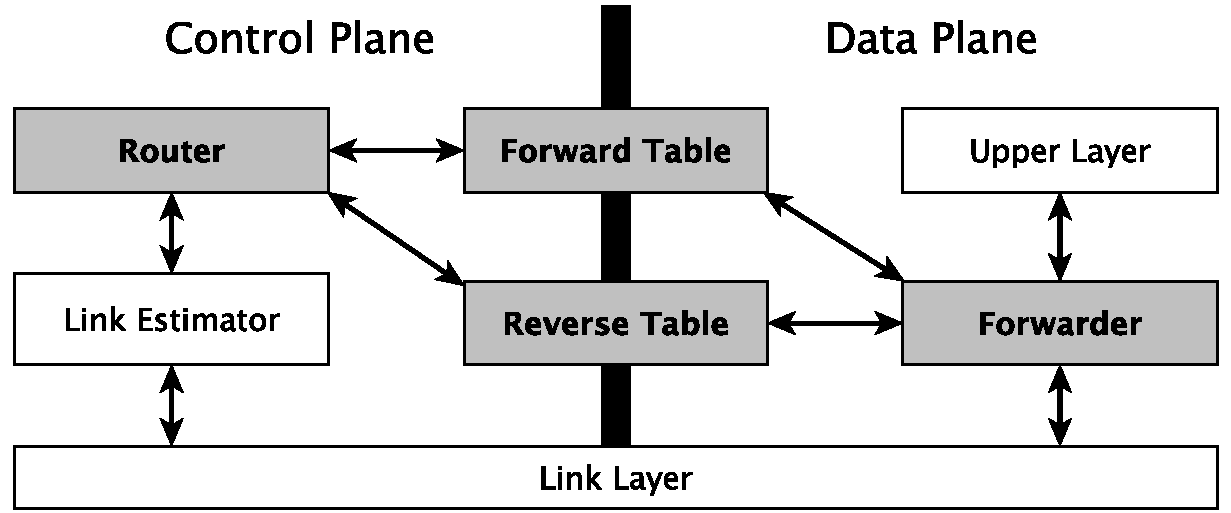
\includegraphics[width=0.8\linewidth]{img/architecture}
} \caption{XCTP architecture.} \label{fig:architecture}
\end{figure}

%--------------------------------
% SUBSEC Changes in data packet %
%--------------------------------
\subsection{Changes in data packet}
\label{sec:changes-in-data-packet}

To allow the navigation of the reverse data packet, we added a $16$
bits packet field to the data packet to represent the address of the
message destination. Figure~\ref{fig:xctp-hdr} shows the new data
packet format. The packet fields are: \textit{P} allows node to
request routing information to other nodes; \textit{C} indicates
congestion notification; \textit{\ac{thl}} each node, when receiving
a packet, increments this field; \textit{\acs{etx}} routing metric
for routes construction and loop detection; \textit{origin} address
of the source node; \textit{destination} address of the destination
node; \textit{seq. num.} sequence number; \textit{collect ID}
collection tree identifier; \textit{Payload} packet data content.

We also created an Acknowledgment (ACK) packet. The ACK packet has a
subset of the data packet fields, as illustrated in
Figure~\ref{fig:ack-pkt}. The \textit{New Features} field $16$ bits
is reserved for future features. The ACK packet is useful as
acknowledgment message for end-to-end transport protocols
implemented over \ac{xctp}.

\begin{figure}[!ht]
\center
    \subfigure[fig:xctp-hdr][Data packet with new destination address field.]{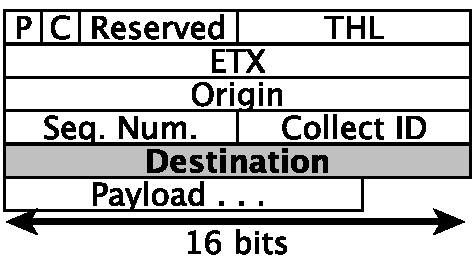
\includegraphics[width=0.40\linewidth]{img/xctp-data-pkt} \label{fig:xctp-hdr}}
    \subfigure[fig:ack-pkt][Acknowledgment Packet.]{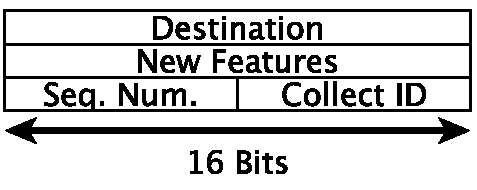
\includegraphics[width=0.40\linewidth]{img/ack-pkt}
    \label{fig:ack-pkt}}
 \caption{Packet formats for XCTP protocol.} \label{fig:pacotes}
\end{figure}




%----------------------
% SUBSEC Reverse Flow %
%----------------------
\subsection{Reverse Flow}
\label{sec:reverse-flow}


\begin{figure*}[!ht]
\centerline{
    \subfigure[fig:a-loop][\ac{xctp} routing tree with reverse flow table.]{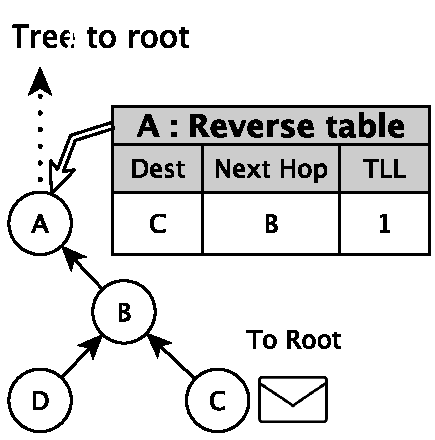
\includegraphics[width=0.17\linewidth]{img/a-loop} \label{fig:a-loop}}
\qquad
    \subfigure[fig:b-loop][Reverse flow table is outdated due to routing loop.]{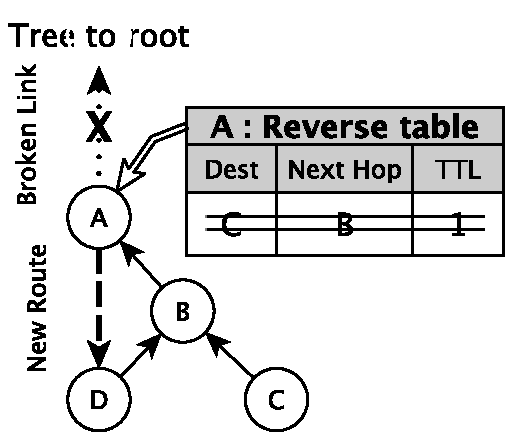
\includegraphics[width=0.2\linewidth]{img/b-loop}\label{fig:b-loop}}
\qquad \qquad
    \subfigure[fig:c-update-link][Reverse flow table before link update.]{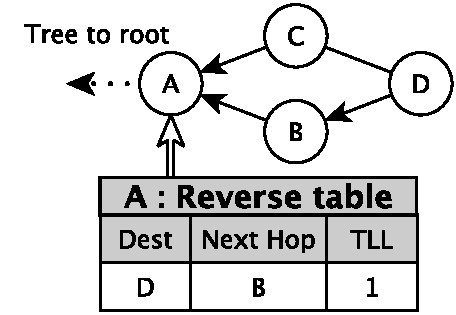
\includegraphics[width=0.2\linewidth]{img/a-update-link}\label{fig:c-update-link}}
\qquad
    \subfigure[fig:d-update-link][Updating reverse flow rule.]{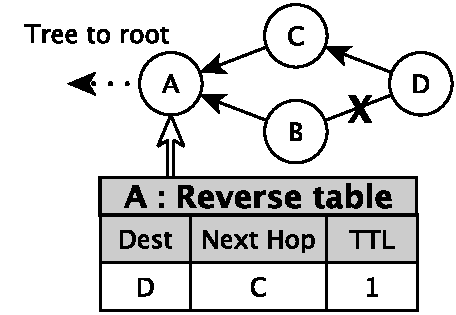
\includegraphics[width=0.2\linewidth]{img/b-update-link}\label{fig:d-update-link}}
} \caption{Control plane reactions over the data plane rules when
detecting a routing loop and updating the routing paths.}
\label{fig:loop}
\end{figure*}

The control plane is responsible for the manipulation of the
\ac{xctp} reverse table. The reverse table has the following fields:
\textit{addr dest}: \ac{xctp} tree descendent (but not 1-hop
neighbor); \textit{next hop}: neighbor address to reach destination;
\textit{\acs{ttl}}: route time to live, where we can apply removing
policies. The Router module implements the basic operations
Creation, Read, Update, and Delete over the reverse table.

\subsubsection{Creation} The table starts empty. When a sensor node forwards a message to the
root, the reverse route is installed. Since the link estimator
module stores information about the 1-hop node neighbors, the router
module does not insert entries in the reverse table of 1-hop
neighbors. Figure~\ref{fig:a-loop} illustrates this situation: where
node C sends data to the root, the intermediate node (that is not a
1-hop neighbor of node C) intercepts the packet from source C and
install a reverse flow.

\subsubsection{Read} Router module provides an interface to query the table. This
mechanism is used for data and control planes. In
Section~\ref{sec:api}, we provide details of using this interface.

\subsubsection{Update e Delete} Router module provides mechanisms for updating and removing
installed rules. These functions are called when there is a topology
change (see Section~\ref{sec:topology-changes}).

There is a trade-off between agility and efficiency regarding the
maintenance of routes in \ac{l2ns}. Agility refers to how fast the
network can react to a topological change, while efficiency is the
energy consumption and the number of packets sent to keep the
network operational. The network requires high frequency of the
beacons to keep routes updated. This increases the agility of the
network but, on the the hand, it reduces efficiency. \ac{ctp} uses
the Trickle algorithm~\cite{trickle} to increase the number of
beacons when the network is unstable and exponentially reduces the
number of beacons when the network is stable, thus keeping a
tradeoff balance between speed and efficiency. \ac{xctp} uses the
data packets to create the reverse route, thus, there is no need for
extra beacons.

%--------------------------
% SUBSEC Topology Changes %
%--------------------------
\subsection{Topology Changes}
\label{sec:topology-changes}

A routing system must know when and where to change the reverse
routes of the data plane so it can correctly react to the network
topology dynamics. \ac{xctp} control plane reacts and changes the
data plane for reverse routes when there is the occurrence of loops
or link failures.

To maintain the consistency of routes, each sensor node keeps the
estimated route cost to the base station. Moreover, this information
is attached to the control and data packets (see
Figure~\ref{fig:xctp-hdr}). \ac{xctp} uses \ac{etx} as the metric
cost. The route cost is always increasing towards the leaf nodes of
the routing tree and this invariant must always be maintained. Loops
are detected when this invariant is broken. In this case, the
reverse flow table entry is removed.


Figures~\ref{fig:a-loop} and \ref{fig:b-loop} illustrate this
situation. In Figure~\ref{fig:a-loop}, we show the initial flow
table. Then, as shown in Figure~\ref{fig:b-loop}, there is a link
failure which causes a loop between nodes A, B, and D. In the event
of a loop, the data plane marks, in the reverse flow table, the
sensor nodes that were descendants and now are parents in the
routing tree. Therefore, the action taken when loops are detected by
\ac{xctp} data plane is to signal the control plane for the loop
detection so that the appropriate reverse flow table entries are
cleared. The reverse flow entries are reconstructed when there are
new data packets in the network.


In case of link exchanges due to the dynamics of link quality, the
control plane must update the data plane reverse flow entries to
reflect this new routing tree configuration. The reverse flow table
is updated when a data packet from an already installed flow is
intercepted but it was routed through a different neighbor.
Figures~\ref{fig:c-update-link} and~\ref{fig:d-update-link}
illustrate this case. Data packets from node D towards the root was
forwarded by node B and changed to be forwarded by node C due to
changes in link quality. Thus, the data plane of node A must be
updated to reflect this new configuration: the reverse flow should
be forwarded by node C.


%-------------
% SUBSEC API %
%-------------
\subsection{API}
\label{sec:api}

Here, we describe the \ac{xctp} Application Programming Interface
(API). The \ac{ctp} protocol does not require a destination address.
\ac{xctp}, on the other hand, needs a destination address to provide
unicast routing to a specific sensor node. \ac{xctp} integrates an
interface that includes the destination address as well as routines
for handling and the reverse and forward tables. The routines are:

\begin{itemize}
    \item \textbf{addr sendTo(target, pkt):} where \textit{target} is the destination address of \ac{xctp} \textit{pkt} packet.
    \item \textbf{addr nextHop(target):} where \textit{target} is an optional parameter. If \textit{target} is instantiated, nextHop(target) routine queries the Reverse Table, otherwise the message is towards the base station.
     \item \textbf{loopDetect():} this routine signals the control plane when a loop is detected (see Section~\ref{sec:topology-changes}).
     \item \textbf{snoopNewPkt(pkt):} when intercepting a data packet from a new flow, the control plane must signal to update the reverse and forward tables.
\end{itemize}

Thus, the interface \textit{sendTo(idNode,pkt)} should be used when
the base station needs to send a packet to a specific node.

Algorithm~\ref{alg:1} describes this routine. On line $1$, we check
if it is a data or acknowledgment packet because only these two
packet types should travel on the reverse path. Then, the
destination address is extracted. If the destination is the node
itself (line $2$), the packet has reached its destination and it
should be properly processed. If the destination is one of its
descendants (line $4$), the packet is forwarded. Otherwise the
recipient is not in any of the routing tables. In this case, there
are two approaches: discard the packet or forward the packet to the
root (line $7$). In the second case, since the root knows the entire
network topology, the root can forward the packet or just discard
it. If the packet does not have a valid address, \ac{xctp} routes
the messages directly to the root (lines $10$-$12$).

\ac{xctp} permits the \textit{any-to-any} communication paradigm.
This is possible due to how the the reverse route is constructed
(line $7$ of Algorithm~\ref{alg:1}). If a node X wants to directly
connected to a node Y, node X can use the routine \textit{sendTo(Y,
pkt)}. Node Y will receive the message from an ancestral of node X
or, in the worst case, the message will go to the root and towards
node Y.

\begin{algorithm}[!t]
    \caption{Internal operation sendTo() interface.}
    \label{alg:1}
    \begin{algorithmic}[1]
        %\REQUIRE $n \geq 0 \vee x \neq 0$
        %\ENSURE $y = x^n$
        
        \IF{$isDataXCTP(pkt)~or~isAckXCTP(pkt)$}
            \IF{$pkt.destination = my.addr$}
                \STATE \textit{// Process package locally.}
            \ELSIF{$pkt.nextHop = nextHop(pkt.dest)$}
                \STATE \textit{// Send unicast message to neighbor in reverse flow.}
            \ELSE
                \STATE \textit{// Drop pkt or forwards to the root.}
            \ENDIF
        \ELSE
            \STATE \textit{// Normally forwards packets through tree \ac{xctp}.}
            \STATE pkt.nextHop = nexHop()
            \STATE forward(pkt)
        \ENDIF
    \end{algorithmic}
\end{algorithm}




%-----------------------------------
% SUBSEC Transport Layer over XCTP %
%-----------------------------------

\subsection{Transport layer over XCTP}
\label{sec:transport-layer-over-xctp}

Using \ac{xctp} API, we implemented a reliable transport protocol,
called \ac{tp}. \ac{tp} uses piggyback and \ac{arq} error-control
mechanism for packet retransmission. Other transport protocols for
\ac{wsn} such as \cite{RCRT, flush, STCP} can also be implemented
over \ac{xctp}. However, the requirement of a few computing
resources and its simplistic implementation were reasons why we
chose this approach in our work.
